\documentclass[aspectratio=16 9,10pt]{beamer}
\usepackage{ctex}
\usepackage{graphicx} 
\usepackage{booktabs}
\usepackage{multicol}
\usepackage{subfig}
\usepackage{xcolor}
\usepackage{tikz}
\usepackage{pgfplots}
\usetheme{Berlin}
\usepackage[english]{babel}
\usepackage[style=authoryear,backend=biber]{biblatex} 
\addbibresource{sn-bibliography.bib}

\title{Advancing Temporal Forecasting: A Comparative Analysis of Conventional Paradigms and Deep Learning Architectures on Publicly Accessible Datasets}
\subtitle{DATS 6501}
\institute{\textbf{George Washington University}}
\author{Liang Gao}


\date{10 December 2024}

\begin{document}
\AtBeginSection[]
{
 \begin{frame}
 \frametitle{List of Content}
 \begin{multicols}{2}
  \tableofcontents[currentsection]
 \end{multicols}
 \end{frame}
}

\begin{frame}
    \titlepage
\end{frame}

\begin{frame}{Content}
\begin{multicols}{2}
    \tableofcontents[hideallsubsections]
\end{multicols}
\end{frame}    
    
\section{Overview}
\begin{frame}{Overview}
    \begin{itemize}
    \item Time-series analysis is a critical area of research with applications spanning diverse
fields such as finance, social science, and climate science.
    \item Numerous models have been developed to address specific problems in these domains.
    \item A noticeable lack of benchmarking studies comparing these models’ performances on standardized datasets.
    \item The primary objective of this study is to evaluate and compare the performance of: 
        \begin{itemize}
        \item Classical models: AR, MA, ARMA, ARIMA
        \item Modern techniques: LSTM, Bi-LSTM, Seq2Seq
        \item State-of-the-Arts: Transformers
        \end{itemize}
    \end{itemize}
\end{frame}


\section{Methodology}
\begin{frame}{Data}
\begin{itemize}
    \item \textbf{Weather Station Beutenberg Dataset} \textcite{weather2020}: Contains meteorological measurements, such as temperature, humidity, and wind speed, recorded every 10 minutes. \textbf{temperature in Celsius}. 
    
    \item \textbf{Power Consumption of Tetouan City} \textcite{power_consumption_of_tetouan_city_849}: Comprises the energy consumption data of Tetouan City, recorded at 10-minute intervals. \textbf{power consumption in Zone 1}.
    
    \item \textbf{Air Pollution Forecasting Dataset} \textcite{kaggle_lstm_dataset}: Hourly measurements of air pollutants along with meteorological features. \textbf{pollution called PM2.5 concentration}.
\end{itemize}
\end{frame}

\begin{frame}{Models: Classical models (\textcite{box2015time})}
\begin{itemize}
    \item \textbf{AR}: Forecast using a linear combination of past values of the variable. AR(\( n_a \)): 
    \[
    y(t) + a_1 y(t-1) + a_2 y(t-2) + \dots + a_{n_a} y(t-{n_a}) = \epsilon(t)
    \]
    
    \item \textbf{MA}: Forecast using past forecast errors. MA(\( n_b \):
    \[
    y(t) = \epsilon(t) + b_1 \epsilon(t-1) + b_2 \epsilon(t-2) + \dots + b_{n_b} \epsilon(t - n_b)
    \]
    
    \item \textbf{ARMA}: Combination of AR and MA models. ARMA(\(n_a, n_b\))
    \[
    y(t) + a_1 y(t-1) + a_2 y(t-2) + \dots + a_{n_a} y(t-{n_a}) = \epsilon(t) + b_1 \epsilon(t-1) + b_2 \epsilon(t-2) + \dots + b_{n_b} \epsilon(t - n_b)
    \]

    \item \textbf{ARIMA}: A generalization of the ARMA model with differencing. ARIMA(\(n_a, d, n_b\)):
    $$
    \left(1+a_1 q^{-1}+\dots+a_{n_a} q^{-n_a}\right)\left(1-q^{-1}\right)^d y(t) = \left(1+b_1 q^{-1}+\dots+b_{n_b} q^{-n_b}\right)\epsilon(t)$$
\end{itemize}
\end{frame}

\begin{frame}{Models: Classical models }
Notation:
\begin{itemize}
    \item \( y(t) \) is the value of the time series at time \( t \),
    \item \( a_1, a_2, \dots, a_{n_a} \) are the coefficients of the AR model,
    \item \( n_a \) is the order of the autoregressive model,
    \item \( b_1, b_2, \dots, b_{n_b} \) are the coefficients of the MA model,
    \item \( n_b \) is the order of the moving average model,
    \item \( \epsilon(t) \) is a white noise normally distributed (WN $\sim (0, \sigma_\epsilon^2)$),
    \item \( d \) is the number of non-seasonal order differencing.
\end{itemize}
\end{frame}


\begin{frame}{Models: Modern techniques}
\begin{itemize}
     \item \textbf{LSTM (\cite{hochreiter1997lstm})}: Long Short-Term Memory: capture long-term dependencies in sequential data while mitigating the vanishing gradient problem 
     \item \textbf{Bi-LSTM (\cite{graves2005framewise}(}: Bidirectional LSTM extends the LSTM by processing data bidirectionally, utilizing forward and backward LSTM to capture past and future context.
     \item \textbf{Seq2Seq (\cite{sutskever2014seq2seq})}: Transform input sequences into output sequences of varying length.
\end{itemize}
\end{frame}

\begin{frame}{State-of-the-art: Transformers}
\begin{itemize}
     \item The Transformers model, introduced by \cite{vaswani2017attention}, has significantly advanced deep learning with its attention mechanism and parallelized architecture. Unlike traditional recurrent models that process sequences sequentially, Transformers handle entire sequences simultaneously, making them more efficient at capturing long-term dependencies.

\end{itemize}
\end{frame}

\begin{frame}{Analysis}
\begin{itemize}
     \item Time series domain knowledge:
        \begin{itemize}
         \item Autocorrelation Function (ACF) and Partial Autocorrelation Function (PACF).
         \item Generalized Partial Autocorrelation (GPAC).
         \end{itemize}
     \item Optuna(\cite{akiba2019optuna}): an open-source hyperparameter optimization framework.

\end{itemize}
\end{frame}

\section{Experiment results}

\begin{frame}{Experiment setting}
\begin{itemize}
\item Optuna: max \( n_a \): 20, max \( n_b \):10, trails: 30

\item Hyperparameters for LSTM, Bi-LSTM, Seq2Seq, and Transformers:
\begin{table}
\centering
\begin{tabular}{lc}
\hline
\textbf{Hyperparameter} & \hspace{3cm} \textbf{Value} \\ \hline
Sequence length         & \hspace{3cm} 6           \\ 
Batch Size              & \hspace{3cm} 128           \\ 
Optimizer               & \hspace{3cm} Adam          \\ 
Training Epochs         & \hspace{3cm} 100           \\ 
Learning Rate           & \hspace{3cm} 0.001         \\ \hline
\end{tabular}
\label{tab:hyperparams}
\end{table}

\item Data was normalized to ensure fair comparison across datasets before calculating evaluation metrics using min-max scaling:
\begin{equation}
\text{X}_{\text{normalized}} = \frac{\text{X} - \text{X}_{\min}}{\text{X}_{\max} - \text{X}_{\min}}.
\end{equation}
\end{itemize}
\end{frame}

\begin{frame}{Exploratory Data Analysis (EDA)}
\begin{figure}
    \centering
    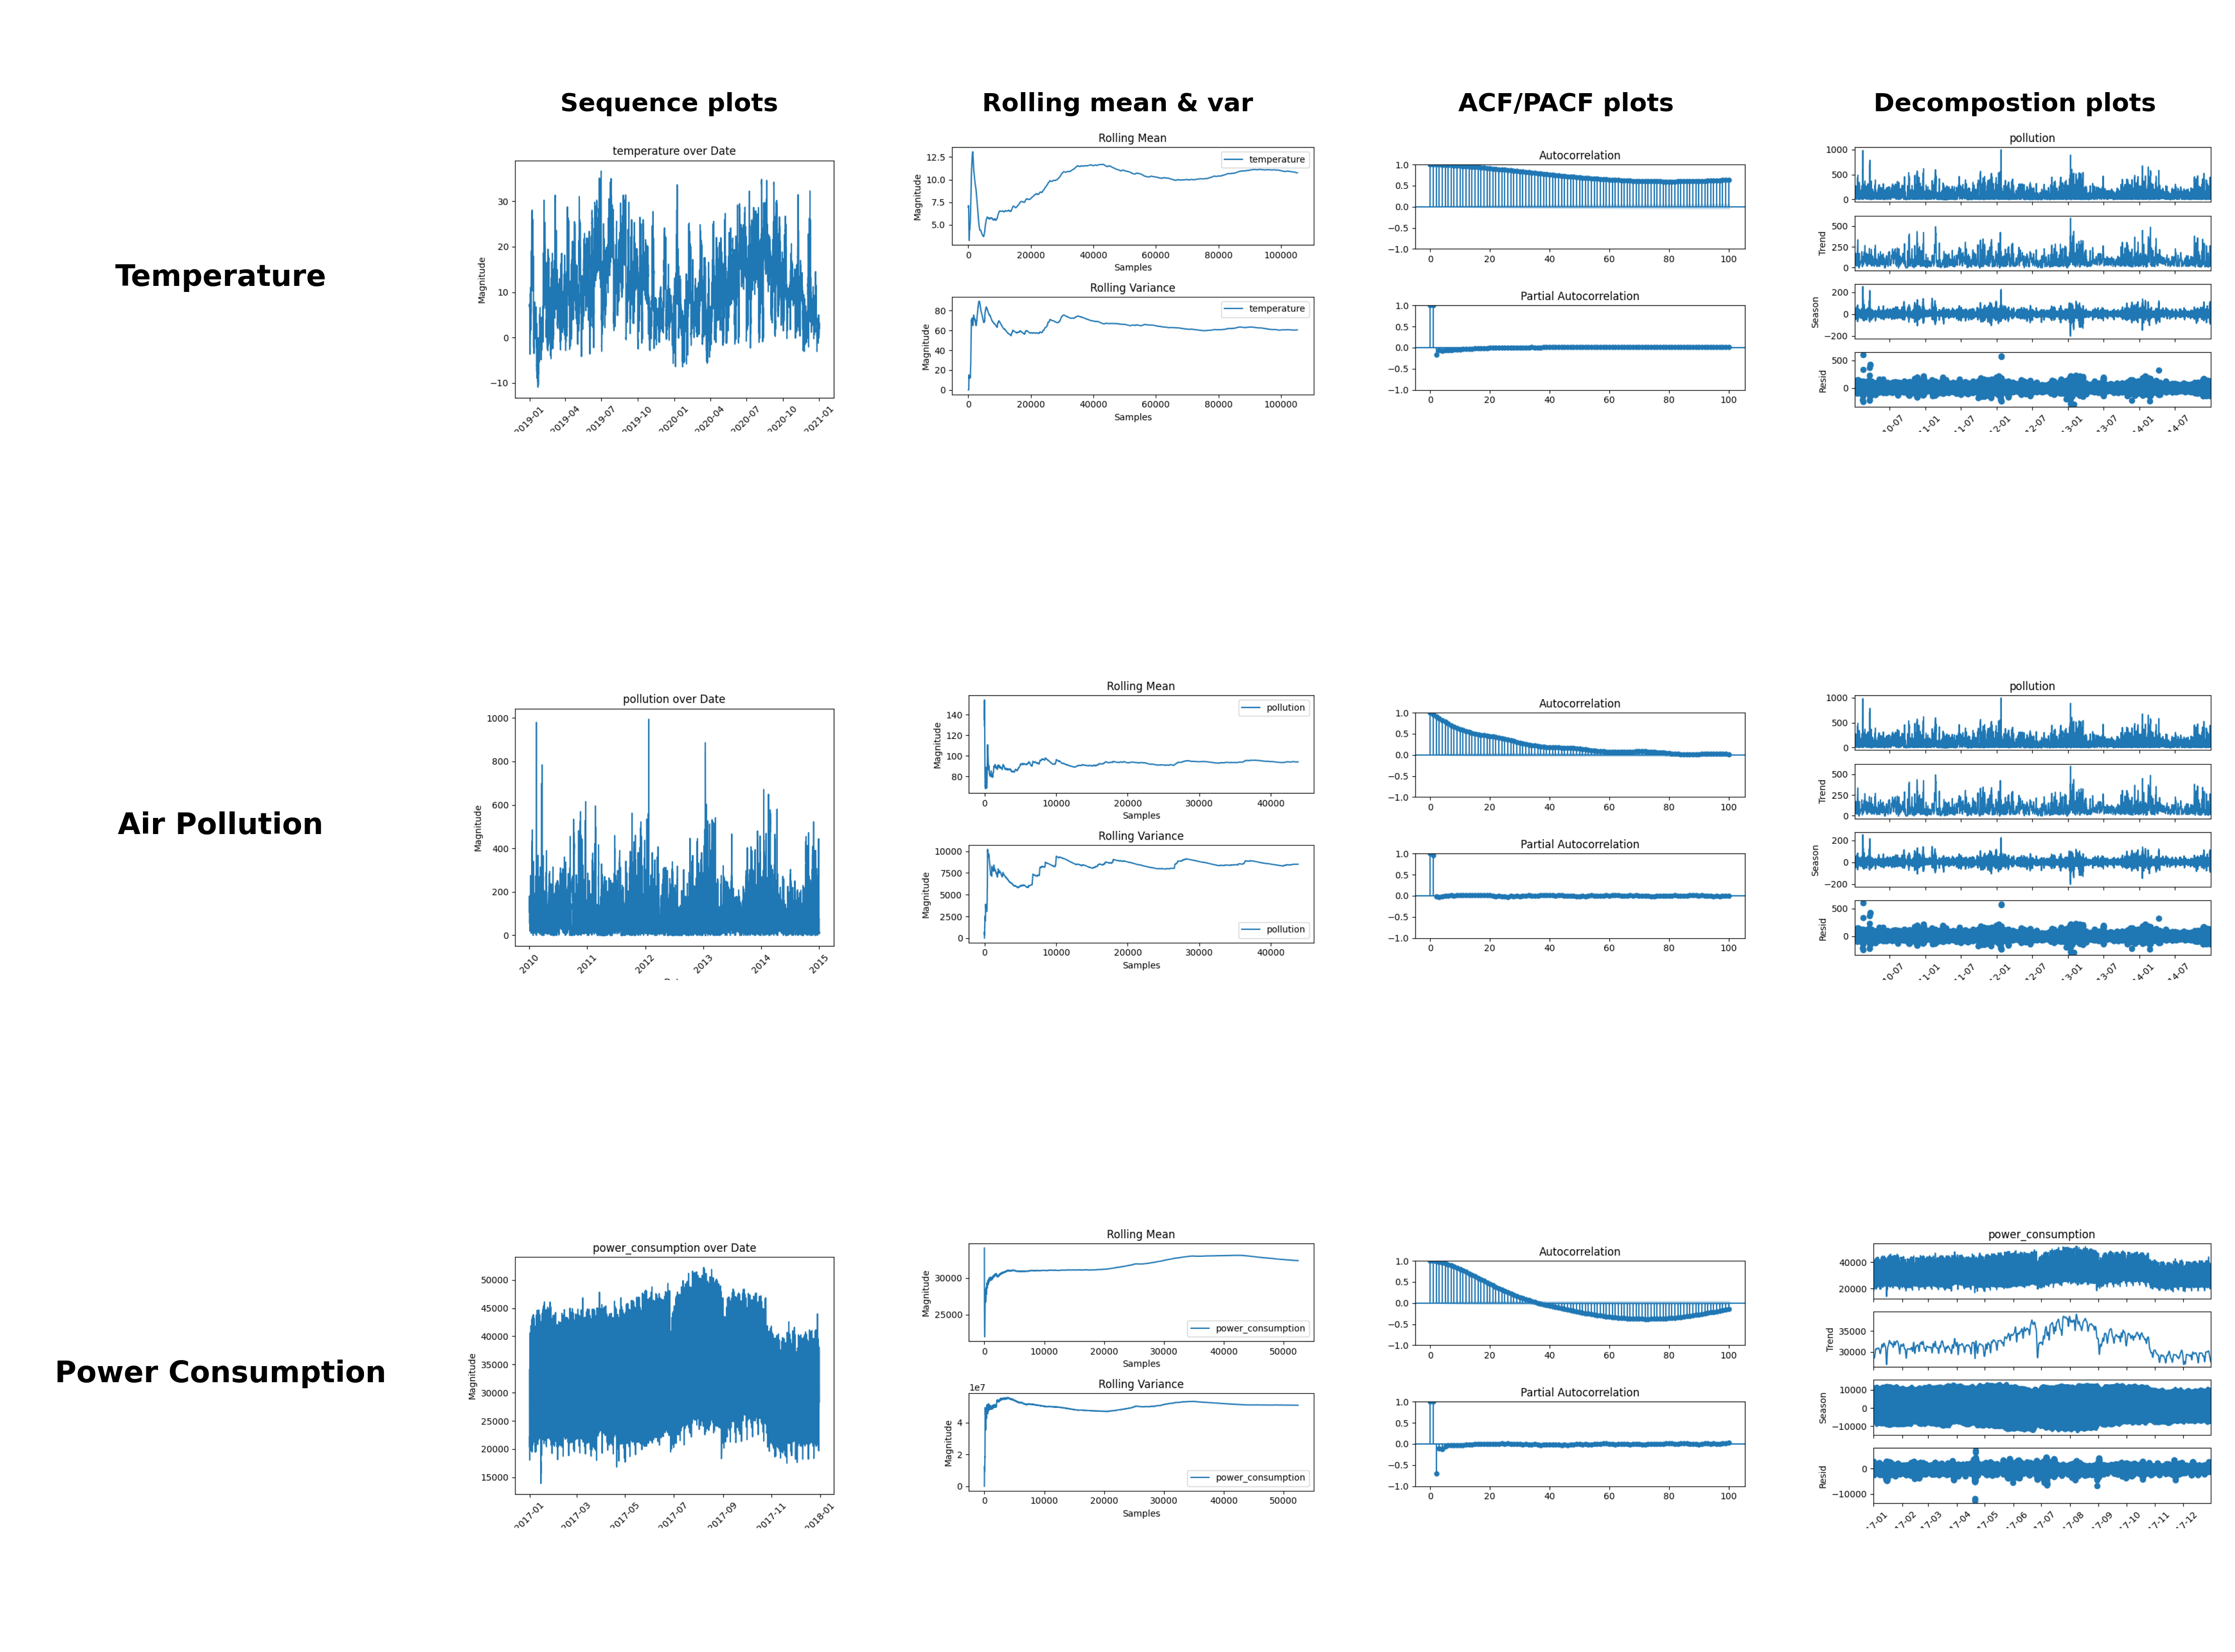
\includegraphics[width=1\textwidth, height=0.8\textheight, keepaspectratio]{eda.pdf}   
    \label{fig:eda_plot}
\end{figure}
\end{frame}

\begin{frame}{Exploratory Data Analysis (EDA)}
\begin{itemize}
 \item Strength of Trend and Seasonality for Each Dataset:
\begin{table}
\centering
\begin{tabular}{lcc}
\hline
\textbf{}        & \textbf{Strength of Trend (\%)} & \hspace{0.5cm}\textbf{Strength of Seasonality (\%)} \\ \hline
Weather                 & 94.33                          & 74.79                                 \\ 
Air Pollution           & 86.01                          & 40.67                                 \\ 
Power Consumption       & 92.41                          & 98.64                                 \\ \hline
\end{tabular}
\end{table}
\end{itemize}

\end{frame}

\begin{frame}{Domain knowledge vs. Optuna}
\begin{itemize}
\item For AR and MA models, we use ACF and PACF plots to find the order
\item For ARMA and ARIMA, we use GPAC.
\end{itemize}
\end{frame}



\begin{frame}{Domain knowledge vs. Optuna}
\begin{itemize}
\item GPAC for three stationary raw datasets to find potential order for ARMA process:
\begin{figure}
	\begin{center}
		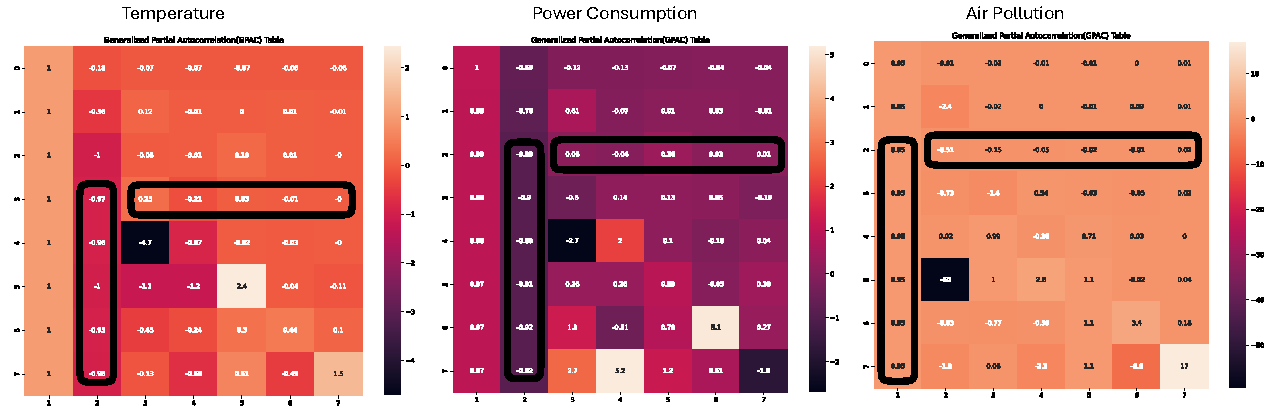
\includegraphics[scale=0.6]{gpac1.pdf}
	\end{center}
	\label{fig:gpac1}
\end{figure}
\end{itemize}
\end{frame}

\begin{frame}{Domain knowledge vs. Optuna}
\begin{itemize}
\item GPAC for three non-seasonal first-order differencing data to find potential order for ARMA process.
\begin{figure}
	\begin{center}
		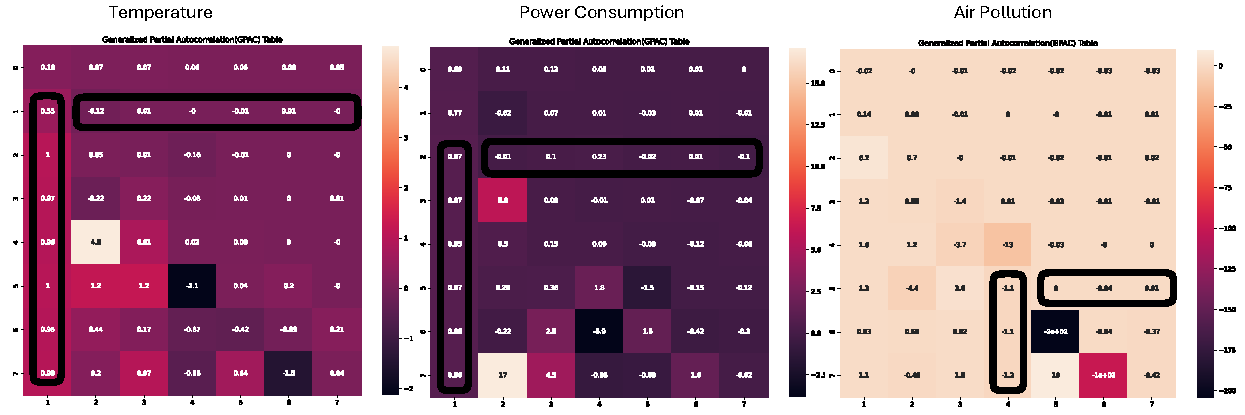
\includegraphics[scale=0.6]{gpac2.pdf}
	\end{center}
	\label{fig:gpac1}
\end{figure}
\end{itemize}
\end{frame}




\begin{frame}{Domain knowledge vs. Optuna}
\begin{table}
\centering
\scalebox{0.8}{
\begin{tabular}{@{}lcccc@{}}
\toprule
\textbf{}               & \textbf{Domain Order}           & \textbf{MSE}     & \textbf{Optuna Order} & \textbf{MSE}     \\ \midrule
\textbf{AR}             &                                 &                  &                       &                  \\
Temperature             & (2)                             & 0.038986         & (4)                   & 0.038950         \\
Power Consumption       & (2)                             & 0.059108         & (10)                  & 0.059213         \\
Air Pollution           & (1)                             & 0.019484         & (5)                   & 0.019482         \\ \midrule
\textbf{MA}               &                                 &                  &                       &                  \\
Temperature             & --                              & --               & (10)                  & 0.038870         \\
Power Consumption       & --                              & --               & (10)                  & 0.059218         \\
Air Pollution           & --                              & --               & (10)                  & 0.019472         \\ \midrule
\textbf{ARMA}             &                                 &                  &                       &                  \\
Temperature             & (2,3)                           & 0.038971         & (8,2)                 & 0.038892         \\
Power Consumption       & (2,2)                           & 0.059206         & (4,5)                 & 0.059281         \\
Air Pollution           & (1,2)                           & 0.019483         & (2,6)                 & 0.019458         \\ \midrule
\textbf{ARIMA}            &                                 &                  &                       &                  \\
Temperature             & (1,1,1)                         & 0.049111         & (7,1,6)               & 0.044493         \\
Power Consumption       & (1,1,2)                         & 0.055292         & (11,1,6)              & 0.055068         \\
Air Pollution           & (4,1,5)                         & 0.019482         & (13,1,10)             & 0.019479         \\ \bottomrule
\end{tabular}
}
\end{table}
\end{frame}

\begin{frame}{Domain knowledge vs. Optuna}
    \begin{itemize}
    \item The minor differences in MSE suggest that while domain knowledge is valuable, Optuna offers a systematic and automated alternative, particularly when prior knowledge is insufficient or when determining an appropriate order is challenging.
    \end{itemize}
\end{frame}



\begin{frame}{Classical models results}
    \begin{itemize}
        \item \textbf{Model Order Selection:}
        \begin{itemize}
            \item Selected the order with the lowest MSE from both domain knowledge and Optuna results.
            \item In cases with multiple GPAC patterns, the order with the lowest MSE was chosen.
        \end{itemize}

        \item \textbf{Findings:}
        \begin{itemize}
            \item The performance of classical models was not very satisfactory, which is expected given their simplicity and reliance on basic approaches.
            \item These models primarily serve as baseline references for comparison.
        \end{itemize}
    \end{itemize}
\end{frame}

\begin{frame}{Classical models results}
\begin{figure}[]
	\begin{center}
       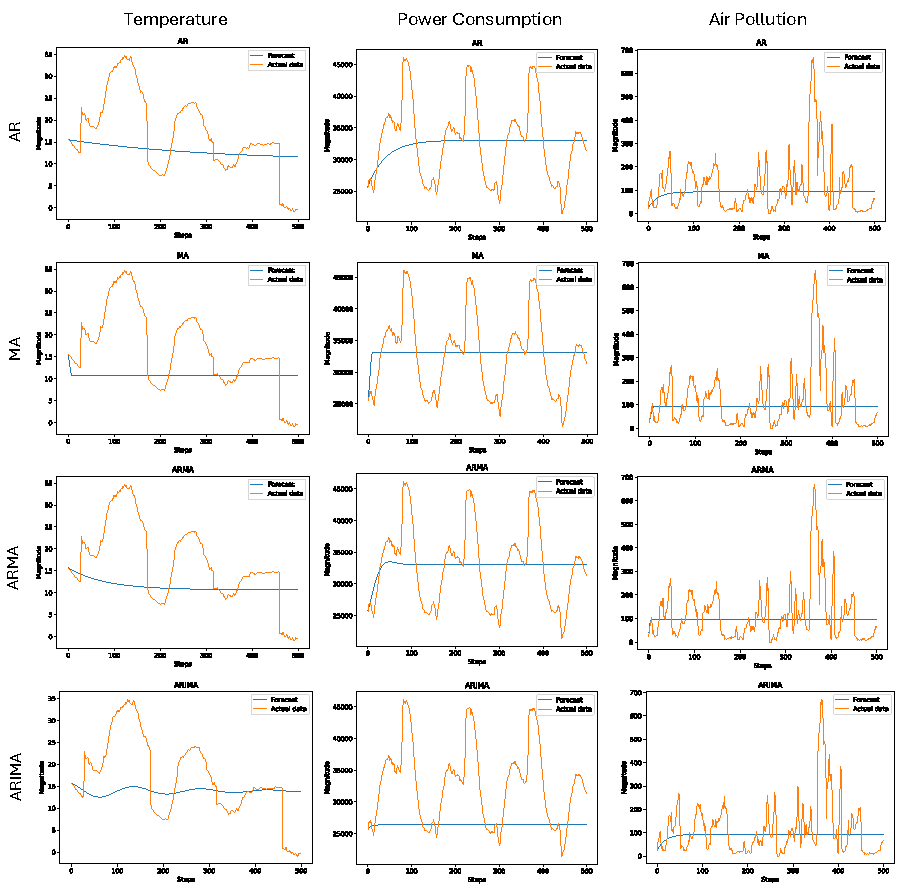
\includegraphics[width=1\textwidth, height=0.8\textheight, keepaspectratio]{classical.pdf} 
	\end{center}
	\label{fig:classical_perf}
\end{figure}
\end{frame}

\begin{frame}{Classical models results}

\begin{table}
\centering
\scalebox{0.8}{
\begin{tabular}{@{}lccc@{}}
\toprule
\textbf{}               & \hspace{0.6cm} \textbf{MSE} & \textbf{RMSE} & \textbf{MAE} \\ \midrule
\textbf{AR}             &              &               &              \\
Temperature             & \hspace{0.6cm}  0.038950     & \hspace{1cm} 0.197359      \hspace{1cm} & 0.161282     \\
Power consumption       & \hspace{0.6cm} 0.059108     & 0.243121      & 0.204268     \\
Air pollution           & \hspace{0.6cm} 0.019482     & 0.139578      & 0.101504     \\ \midrule
\textbf{MA}             &              &               &              \\
Temperature             & \hspace{0.6cm} 0.038870     & 0.197156      & 0.160967    \\
Power consumption       & \hspace{0.6cm} 0.059218     & 0.243347      & 0.204480     \\
Air pollution           & \hspace{0.6cm} 0.019472     & 0.139542      & 0.101515     \\ \midrule
\textbf{ARMA}           &              &               &              \\
Temperature             & \hspace{0.6cm} 0.038892     & 0.197210      & 0.161051     \\
Power consumption       & \hspace{0.6cm} 0.059206     & 0.243322      & 0.204456     \\
Air pollution           & \hspace{0.6cm} 0.019458     & 0.139493      & 0.101845      \\ \midrule
\textbf{ARIMA}          &              &               &              \\
Temperature             & \hspace{0.6cm} 0.044493     & 0.210933      & 0.178464     \\
Power consumption       & \hspace{0.6cm} 0.055068     & 0.234666      & 0.193346     \\
Air pollution           & \hspace{0.6cm} 0.019479     & 0.139569      & 0.101566       \\ \bottomrule
\end{tabular}
}
\end{table}
\end{frame}


\begin{frame}{Modern techniques results}
    \begin{itemize}
        \item \textbf{Training Setup:}
        \begin{itemize}
            \item All models were trained with identical hyperparameters.
            \item This ensures direct comparability across models and isolates the impact of each model's architecture.
        \end{itemize}

        \item \textbf{Findings:}
        \begin{itemize}
            \item The modern techniques significantly outperformed classical models, with lower MSE values and superior accuracy.
            \item Among the models, LSTM, despite its simpler architecture, achieved the lowest MSE, indicating its effectiveness for the datasets in this study.
        \end{itemize}
    \end{itemize}
\end{frame}


\begin{frame}{Modern techniques results}
\begin{table}[h]
\centering
\scalebox{0.8}{
\begin{tabular}{@{}lccc@{}}
\toprule
\textbf{}               & \hspace{0.6cm} \textbf{MSE} & \textbf{RMSE} & \textbf{MAE} \\ \midrule
\textbf{LSTM}           &              &               &              \\
Temperature             & \hspace{0.6cm} 0.000127     & \hspace{1cm} 0.011277      \hspace{1cm} & 0.004017     \\
Power consumption       & \hspace{0.6cm} 0.000175     & 0.013225      & 0.008923     \\
Air pollution           & \hspace{0.6cm} 0.001260     & 0.035502      & 0.018459     \\ \midrule
\textbf{Bi-LSTM}        &              &               &              \\
Temperature             & \hspace{0.6cm} 0.000131     & 0.011437      & 0.004310     \\
Power consumption       & \hspace{0.6cm} 0.000179     & 0.013362      & 0.009071     \\
Air pollution           & \hspace{0.6cm} 0.000261     & 0.035516      & 0.019128     \\ \midrule
\textbf{Seq2Seq}        &              &               &              \\
Temperature             & \hspace{0.6cm} 0.000128     & 0.011307      & 0.004099     \\
Power consumption       & \hspace{0.6cm} 0.000226     & 0.015046      & 0.009872     \\
Air pollution           & \hspace{0.6cm} 0.000247     & 0.035312      & 0.018662       \\ \bottomrule
\end{tabular}
}
\end{table}
\end{frame}




\begin{frame}{Modern techniques results}
\begin{figure}[]
	\begin{center}
	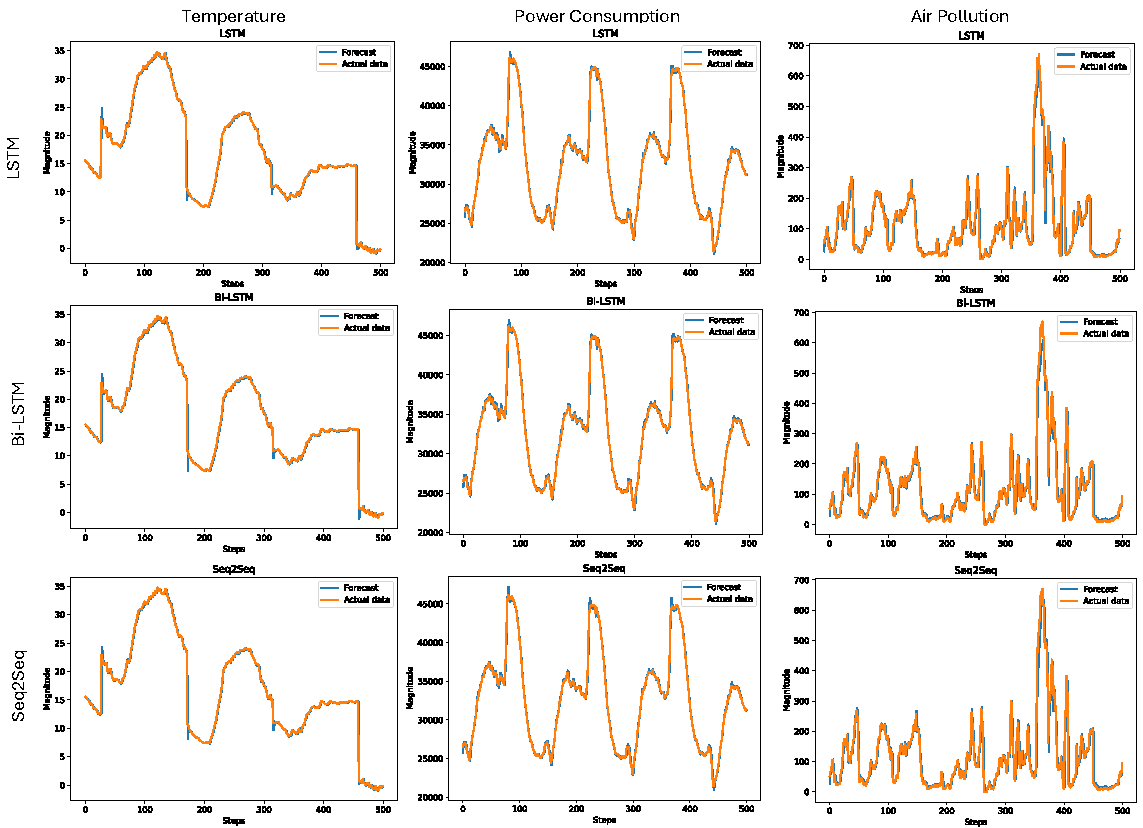
\includegraphics[width=1\textwidth, height=0.8\textheight, keepaspectratio]{modern.pdf}
	\end{center}
\end{figure}
\end{frame}


\begin{frame}{State-of-the-art results}
    \begin{itemize}
        \item \textbf{Training Setup:}
        \begin{itemize}
            \item Used the same hyperparameters as the modern techniques, to ensure consistency.
        \end{itemize}

        \item \textbf{Findings:}
        \begin{itemize}
            \item The Transformer model outperforms the classical models.
            \item However, it does not exceed the performance of the three modern techniques (LSTM, BiLSTM, Seq2Seq).
            \item This suggests that for these three datasets, the complex Transformer architecture may not be necessary for optimal performance.
        \end{itemize}
    \end{itemize}
\end{frame}

\begin{frame}{State-of-the-art results}
\begin{table}
\centering
\begin{tabular}{@{}lccc@{}}
\toprule
\textbf{}               & \hspace{0.6cm} \textbf{MSE} & \textbf{RMSE} & \textbf{MAE} \\ \midrule
% \textbf{Transformers}    &              &               &              \\
Temperature           & \hspace{0.6cm} 0.000599     & \hspace{1cm} 0.024466     \hspace{1cm} & 0.016530     \\
Power consumption       & \hspace{0.6cm} 0.000467     & 0.021602      & 0.015685     \\
Air pollution           & \hspace{0.6cm} 0.001370     & 0.037011      & 0.019526     \\ \bottomrule
\end{tabular}
\end{table}

\end{frame}

\begin{frame}{State-of-the-art results}
\begin{figure}[]
	\begin{center}
	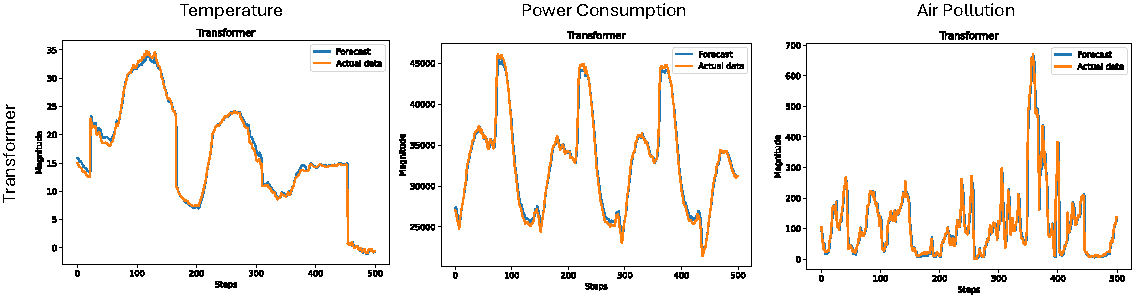
\includegraphics[width=1\textwidth, height=0.8\textheight, keepaspectratio]{trans.pdf}
	\end{center}
\end{figure}

\end{frame}

\section{Conclusion}
\begin{frame}{Conclusion}
    \begin{itemize}
        \item \textbf{Models Evaluated:}
        \begin{itemize}
            \item Classical Models: AR, MA, ARMA, ARIMA
            \item Modern Techniques: LSTM, BiLSTM, Seq2Seq
            \item State-of-the-Art: Transformers
        \end{itemize}
        
        \item \textbf{Performance Comparison:}
        \begin{itemize}
            \item Modern techniques and Transformers consistently outperformed classical models.
            \item LSTM, with its simplest architecture, achieved the lowest MSE.
        \end{itemize}
        
        \item \textbf{Insights:}
        \begin{itemize}
            \item Even the simplest deep learning architectures are sufficient to handle these datasets effectively.
        \end{itemize}
    \end{itemize}
\end{frame}

\section{Limitations}
\begin{frame}{Limitations}
    \begin{itemize}
        \item \textbf{Classical Models:}
        \begin{itemize}
            \item Simple configurations were selected based on available information, which may not represent the optimal performance.
            \item Further exploration could lead to better-performing classical models.
        \end{itemize}
        
        \item \textbf{GPAC:}
        \begin{itemize}
            \item Limited the number of rows and columns, which may have prevented us from identifying the correct patterns.
        \end{itemize}
        
        \item \textbf{Optuna Hyperparameter Tuning:}
        \begin{itemize}
            \item Maximum potential order and number of trials were constrained, limiting the discovery of more suitable models.
        \end{itemize}
        
        \item \textbf{Modern Techniques and Transformers:}
        \begin{itemize}
            \item All models were trained with a fixed sequence length and common hyperparameters, which may not be optimal for every model or dataset.
        \end{itemize}
    \end{itemize}
\end{frame}

\section{Future Work}
\begin{frame}{Future Work}
    \begin{itemize}
        \item \textbf{SARIMA Models:}
        \begin{itemize}
            \item Implement Seasonal Autoregressive Integrated Moving Average (SARIMA) models \cite{box2015time} to capture seasonality more effectively.
        \end{itemize}
        
        \item \textbf{Box-Jenkins Methodology:}
        \begin{itemize}
            \item Apply the advanced Box-Jenkins methodology \cite{box2015time} for more comprehensive performance comparisons.
        \end{itemize}
        
        \item \textbf{Model Variations:}
        \begin{itemize}
            \item Explore other model variations to further refine the findings and broaden the scope of the research.
        \end{itemize}

       \item \textbf{Expanding to Multivariate Time Series:}
        \begin{itemize}
            \item Currently, the analysis focuses on univariate time series. Future work could extend the models to multivariate time series analysis to capture relationships between multiple variables over time.
        \end{itemize}
    \end{itemize}
\end{frame}

\begin{frame}[allowframebreaks]{References}
\printbibliography
\end{frame}

\end{document}
